% !TEX program = xelatex
% ETF 动量轮动策略 · 研究分析报告
% 内容与 web/templates/analysis.html 同步；编译: lualatex analysis_report.tex (需 ctex/fandol)
\documentclass[11pt]{ctexart}

\usepackage[a4paper,margin=2.4cm]{geometry}
\usepackage{amsmath}
\usepackage{booktabs}
\usepackage{threeparttable}
\usepackage{tabularx}
\usepackage{longtable}
\usepackage{multirow}
\usepackage{makecell}
\usepackage{graphicx}
\usepackage{xcolor}
\usepackage{enumitem}
\usepackage{titlesec}
\usepackage{caption}
\usepackage{fancyhdr}
\usepackage{lastpage}
\usepackage[hidelinks]{hyperref}

\definecolor{accent}{HTML}{C0392B}
\definecolor{poscol}{HTML}{1E8449}

\captionsetup{font=small,labelfont=bf,skip=6pt}
\setlist{nosep,leftmargin=2.2em,itemsep=2pt}

\titleformat{\section}{\Large\bfseries}{\thesection}{0.8em}{}
\titleformat{\subsection}{\large\bfseries}{\thesubsection}{0.8em}{}
\titleformat{\subsubsection}{\normalsize\bfseries}{\thesubsubsection}{0.8em}{}

\graphicspath{{figs/}}

% —— 页眉页脚 ——
\pagestyle{fancy}
\fancyhf{}
\fancyhead[L]{\small\itshape ETF 动量轮动策略 · 研究分析报告}
\fancyhead[R]{\small 数据截止 2026-08-20}
\fancyfoot[C]{\small 第 \thepage\ 页 / 共 \pageref{LastPage} 页}
\renewcommand{\headrulewidth}{0.4pt}

\newcommand{\pos}[1]{\textcolor{poscol}{#1}}   % 正收益
\newcommand{\red}[1]{\textcolor{accent}{#1}}   % 负收益/回撤

\title{\bfseries ETF 动量轮动策略：研究分析报告\\[0.4em]
\large 十年样本上的机制分解、参数稳健性与样本外验证}
\author{\normalsize ETF 动量轮动策略项目组}
\date{\normalsize 数据截止 2026-08-20\quad 报告生成 2026-08-25}

\begin{document}

\maketitle
\thispagestyle{fancy}

\begin{abstract}
\noindent 本报告系统总结「窄池相对动量 + regime filter + 两端风控模块」三层信号堆栈的十年回测证据。
策略在纳指(513100)、黄金(518880)、创业板(159915)三只 ETF 上做 20 日相对动量轮动，日频全仓持有动量最强标的，
核心风控为「上证指数动量超过池内最强 $\rightarrow$ 空仓」的 regime filter，辅以相对/绝对止损、加速止盈（动量过热止盈）与恐慌抄底。
样本区间为 2016-07-07 至 2026-08-20（约 10.1 年）。
\end{abstract}

\tableofcontents
\clearpage

% ═══════════════ 1 摘要 ═══════════════
\section{摘要}

\begin{center}
\begin{tabular}{lrlr}
\toprule
累计收益 & \pos{3785\%} & 年化收益 & 45.51\% \\
最大回撤 & \red{$-18.08\%$} & Calmar & 2.52 \\
Sharpe & 1.73 & 年化波动率 & 23.19\% \\
交易笔数(买+卖) & 253 & 负收益年份数 & 1 \\
\bottomrule
\end{tabular}
\end{center}

同期\textbf{等权买入持有}三只 ETF：累计 283\%、年化 14.74\%、最大回撤 \red{$-20.15\%$}、Calmar 0.73。
策略以相近的最大回撤（$-18.08\%$ vs $-20.15\%$）取得约 10 倍的累计收益。

核心结论：
\begin{enumerate}
  \item 收益来自「窄池相对动量 + regime filter + 两端风控模块」三层信号堆栈：消融显示上证空仓、加速止盈、恐慌抄底、绝对止损、快速通道、QQQ 混合动量\textbf{均为独立正贡献}，删除任一模块年化/Calmar 双降。
  \item 除动量周期外，其余参数在邻域内整体稳健（无悬崖式劣化）；个别档位略优/略劣，均不构成换参理由。
  \item 动量周期曲线在\textbf{当前引擎口径下为 18$\sim$22 日的缓坡}（全样本最优 19 日 Calmar 2.52，20 日排第 1/21 名）——旧口径下的「20/21 孤峰」已消失；但两半窗口中最优值从 19 漂移到 22，\textbf{参数漂移真实存在}。
  \item 样本外验证窗（2021-08 起）年化 43.94\%、Calmar 2.40，与全样本基本持平；长样本（2015 起）年化 45.74\%。考虑到 2025--26 年黄金/纳指极端行情不可复制，长期年化的诚实预期区间为 \textbf{30\%$\sim$45\%}、回撤 $-18\%\sim-25\%$。
\end{enumerate}

% ═══════════════ 2 引言 ═══════════════
\section{引言：策略在动量轮动谱系中的位置}

\subsection{经典动量轮动策略对比}

\begin{table}[htbp]
\centering
\caption{与经典动量轮动策略的谱系对比}
\begin{tabularx}{\textwidth}{p{3.4cm}XXp{2.2cm}X}
\toprule
策略 & 信号 & 调仓频率 & 持仓 & 下跌保护 \\
\midrule
GEM (Antonacci) & 12 个月收益：相对+绝对动量 & 月频 & 全仓 1 只 & 绝对动量为负 $\rightarrow$ 切债券 \\
DAA (Keller) & 13612W 多周期加权动量 & 月频 & Top-3 等权 & 按坏资产数量比例切防御 \\
VAA (Keller) & 风险调整动量(动量/波动率) & 月频 & Top-4 等权 & 有坏资产 $\rightarrow$ 全仓防御 \\
TSMOM (Moskowitz) & 12 个月时序动量符号 & 月频 & 多资产独立信号 & 负动量空仓+波动率缩放 \\
\addlinespace
\textbf{本策略} & 20 日相对动量排名 & 日频 & 全仓 1 只 & 上证空仓 filter + 止损 + 加速止盈 + 恐慌抄底 \\
\bottomrule
\end{tabularx}
\end{table}

本策略可视为 \textbf{GEM 的高频变体}：以日频替代月频、20 日替代 12 个月、上证 regime filter 替代逐标的绝对动量门。
与文献中月频动量系统相比，它把「趋势跟踪」压缩到约一个月的形成期——这是收益来源，也是脆弱性来源（见第 \ref{sec:fragile} 节）。

\subsection{信号堆栈：相互独立的风险收益来源}

本策略不是单一动量策略，而是一个\textbf{信号堆栈}，各模块在市场不同状态分别开火：

\begin{table}[htbp]
\centering
\caption{信号堆栈的模块、触发条件与理论角色}
\begin{tabularx}{\textwidth}{p{3.2cm}XXX}
\toprule
模块 & 触发条件(简化) & 理论角色 & 主导市况 \\
\midrule
20 日相对动量排名 & 持有 mom20 最高的标的 & 横截面动量(alpha 引擎) & 趋势市 \\
上证空仓 filter & 上证 mom20 $>$ 池内最强 $\rightarrow$ 空仓+3 天冷却 & Regime filter / 领导力背离 & 系统性风险、风格切换 \\
快速通道 & 挑战者动量领先 $\ge3\%$ 且确认 2 天 $\rightarrow$ 立即切换 & 趋势加速器 / 崩盘逃生口 & 急涨急跌 \\
止损 + 绝对止损 & 有更优候选且 pnl$\le-5\%$ 切换；仍第一但 pnl$\le-5\%$ 清仓 & 尾部截断 & 单边下跌 \\
加速止盈 & mom10 $>$ 自身历史 $\mu+3\sigma$ $\rightarrow$ 清仓(黄金止盈后冷却 3 天) & 均值回归叠加：卖过热 & 冲顶 / blow-off \\
恐慌抄底 & 指数 mom10 $<\mu-2.5\sigma$ 且 $<$ MA200 $\rightarrow$ 买创业板锁仓 7 天 & 逆向叠加：买恐慌 & 恐慌底 \\
确认天数/最短持有/动量差 & 2 天确认、10 天最短持有、$\ge1\%$ 动量差 & 换手与 whipsaw 成本控制 & 全程 \\
\bottomrule
\end{tabularx}
\end{table}

一句话概括：\textbf{趋势跟踪为体、regime filter 为锚、两端（过热/恐慌）均值回归叠加为辅}。
三类信号低相关、分时开火，策略的稳健性来自这种集成结构而非任何单一参数。

% ═══════════════ 3 方法与数据 ═══════════════
\section{方法与数据}

\subsection{决策顺序（优先级即实现顺序）}

\begin{enumerate}
  \item 更新净值并计算排名分数（mom20，纳指为 $0.3\times513100 + 0.7\times\text{QQQ-CNY}$ 混合动量）；
  \item \textbf{恐慌抄底}：创业板指或上证指数 mom10 跌破自身历史 $\mu-2.5\sigma$ 且价格 $<$ MA200 $\rightarrow$ 买入创业板，锁仓 7 天（期间仅允许止损退出）；
  \item \textbf{上证空仓}：上证 mom20 高于池内最强标的 $\rightarrow$ 清仓到空仓，再入场需等 3 天冷却；
  \item 空仓入场：候选动量 $\ge3\%$ 当日即买（$>3\%$ 即买），否则需连续 2 天第一（确认买入）；
  \item 持仓切换：止损（有更优候选且 pnl$\le-5\%$）$\rightarrow$ 排名确认后快速通道（momentum gap $\ge3\%$）$\rightarrow$ 正常切换（$\ge1\%$，持有$\ge10$ 天）；
  \item \textbf{绝对止损}：持仓仍是动量第一但 pnl$\le-5\%$ $\rightarrow$ 清仓（2026-06 纳指 $-9.79\%$ 事件的修复项）；
  \item \textbf{加速止盈}：持仓 mom10 $>$ 自身历史 $\mu+3\sigma$ $\rightarrow$ 清仓；黄金止盈后 3 天内禁止买回（2026-08-18 决议）。
\end{enumerate}

成本口径：每笔卖出/买入各扣 0.01\% 手续费（commission=0.0001），默认零滑点；信号日\textbf{收盘价成交}，当日收益归旧仓，无前视。

\subsection{数据与口径}

\begin{itemize}
  \item \textbf{行情}：Tushare 日线（三只 ETF + 上证指数 000001.SH + 创业板指 399006.SZ），分红拆分按复权因子现场重算；回测起点前预热 320 自然日保证 MA200 就绪。
  \item \textbf{纳指动量混合}：排名与阈值用 $(1-0.7)\times513100 + 0.7\times\text{QQQ}\times\text{USDCNY}$ 的动量（净值与止损仍按 513100 成交价），以消除 QDII 溢价与申赎扰动；美国数据对齐采用「CN 日 D 只用美国 $\le$D$-$1 收盘」，严格无前视。
  \item \textbf{停牌与缺失}：价格 NaN $\rightarrow$ 动量 NaN $\rightarrow$ 不参与排名；持仓停牌日净值冻结、不成交。
  \item \textbf{评估指标}：年化收益 $= \text{NAV}^{252/\text{交易日数}}-1$；最大回撤与 Calmar 基于日频净值；Sharpe 基于日收益年化。
\end{itemize}

复现命令：
\begin{quote}\small\ttfamily
curl -X POST http://127.0.0.1:8082/api/bt/run \\
\quad{} -H 'Content-Type: application/json' \\
\quad{} -d '\{"universe":"纳指,黄金,创业","start\_date":"2016-07-07", \\
\quad{}\phantom{ -d '}"end\_date":"2026-08-20"\}'
\end{quote}

% ═══════════════ 4 结果 ═══════════════
\section{结果}

\subsection{基线业绩与回撤结构}

\begin{figure}[htbp]
\centering
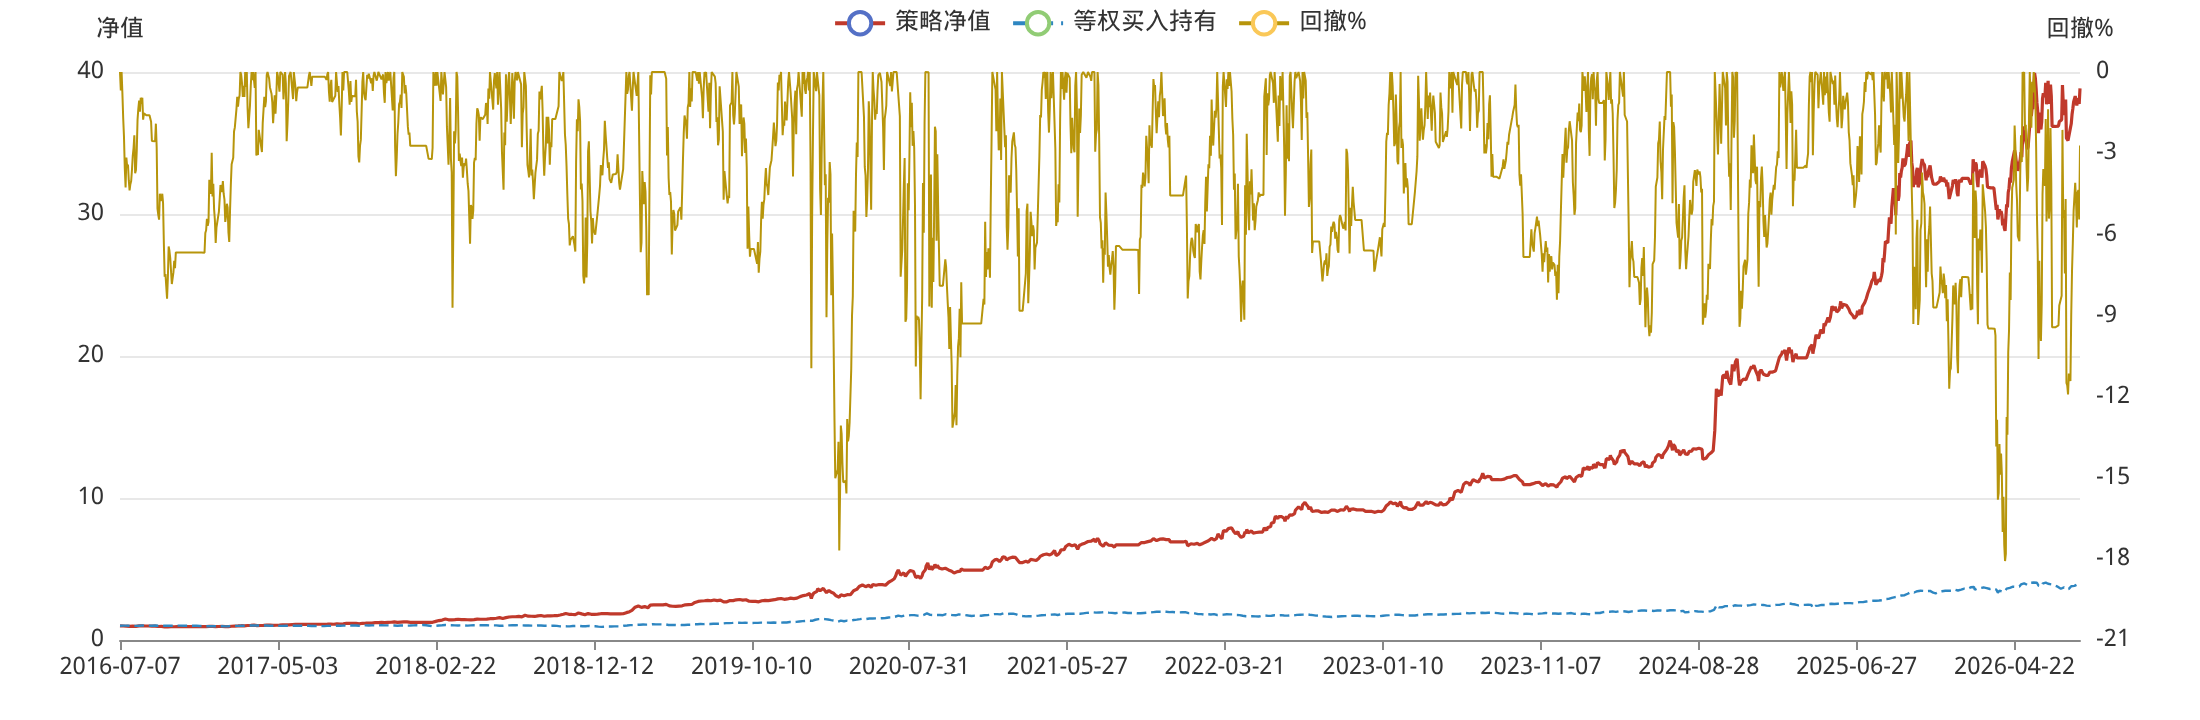
\includegraphics[width=\textwidth]{nav.png}
\caption{策略净值 vs 等权买入持有（下轴为回撤\%，2016-07-07 至 2026-08-20）}
\end{figure}

\subsubsection{年度收益}

\begin{table}[htbp]
\centering
\caption{分年度收益（主样本）}
\begin{tabular}{rrrr}
\toprule
年份 & 收益 & 年份 & 收益 \\
\midrule
2016 & \red{$-5.30\%$} & 2022 & \pos{+31.30\%} \\
2017 & \pos{+32.40\%} & 2023 & \pos{+26.60\%} \\
2018 & \pos{+47.95\%} & 2024 & \pos{+62.03\%} \\
2019 & \pos{+59.35\%} & 2025 & \pos{+68.08\%} \\
2020 & \pos{+78.95\%} & 2026 & \pos{+24.30\%} \\
2021 & \pos{+30.53\%} & & \\
\bottomrule
\end{tabular}
\end{table}

11 个年份中仅 2016 年（$-5.30\%$）为负。

\subsubsection{回撤事件（$>10\%$）}

\begin{table}[htbp]
\centering
\caption{十年间深度超过 10\% 的回撤事件}
\begin{tabular}{clrrrrr}
\toprule
\# & 峰值 $\rightarrow$ 谷底 & 深度 & 下跌耗时 & 修复日 & 修复耗时 \\
\midrule
1 & 2020-01-22 $\rightarrow$ 2020-02-03 & \red{$-10.95\%$} & 2 天 & 2020-02-06 & 3 天 \\
2 & 2020-02-24 $\rightarrow$ 2020-03-23 & \red{$-17.69\%$} & 20 天 & 2020-04-27 & 24 天 \\
3 & 2020-07-03 $\rightarrow$ 2020-08-20 & \red{$-12.1\%$} & 34 天 & 2020-08-28 & 6 天 \\
4 & 2020-09-02 $\rightarrow$ 2020-10-27 & \red{$-13.16\%$} & 33 天 & 2021-01-04 & 48 天 \\
5 & 2025-09-29 $\rightarrow$ 2026-04-03 & \red{$-18.08\%$} & 120 天 & 2026-05-11 & 22 天 \\
6 & 2026-05-29 $\rightarrow$ 2026-07-30 & \red{$-11.92\%$} & 43 天 & 未修复 & — \\
\bottomrule
\end{tabular}
\end{table}

十年间 6 次回撤超过 10\%：其中 4 次集中在 2020 年（疫情冲击、黄金见顶、止盈空转）；
第 5 次（2025-09-29 $\rightarrow$ 2026-04-03）为全样本最深（\red{$-18.59\%$}，下跌 120 个交易日）；
第 6 次（2026-05-29 $\rightarrow$ 2026-07-30）深度 $-11.92\%$，期末仍未完全修复（当前 $-2.72\%$）。
旧版分析中「2026-06$\sim$07 连环止损段 $-25.7\%$（旧参数口径、十年最深）」在当前默认参数（QQQ 混合动量 + 黄金止盈冷却）下已收敛至 $-11.92\%$——两次默认参数变更对尾部风险的实际改善。

\subsection{模块消融：每个模块的独立贡献}

固定其余参数、逐一关闭/回退单个模块，与基线比较（$\Delta$ 为相对基线的变化）：

\begin{table}[htbp]
\centering
\caption{模块消融结果（回退方向即「关掉/还原该默认开关」）}
\small
\begin{tabularx}{\textwidth}{Xrrrrl}
\toprule
开关(回退方向) & 年化 & 最大回撤 & Calmar & 交易 & 判定 \\
\midrule
\textbf{基线(当前默认参数)} & \textbf{45.51\%} & \textbf{$-18.08\%$} & \textbf{2.52} & 253 & — \\
上证空仓 regime filter & 40.75\% ($-4.76$pp) & $-19.88\%$ & 2.05 ($-0.47$) & 219 & 负优化 \\
恐慌抄底 & 42.45\% ($-3.06$pp) & $-18.08\%$ & 2.35 ($-0.17$) & 243 & 负优化 \\
加速止盈 & 41.47\% ($-4.04$pp) & $-25.50\%$ & 1.63 ($-0.89$) & 189 & 负优化 \\
绝对止损 & 43.88\% ($-1.63$pp) & $-21.53\%$ & 2.04 ($-0.48$) & 243 & 负优化 \\
止盈冷却 3 天(仅黄金) & 47.32\% (+1.81pp) & $-17.69\%$ & 2.67 (+0.15) & 264 & 正贡献(回退) \textsuperscript{①} \\
止盈冷却扩至全部标的 & 38.51\% ($-7.00$pp) & $-20.78\%$ & 1.85 ($-0.67$) & 258 & 负优化 \\
止盈冷却 5 天 & 44.76\% ($-0.75$pp) & $-26.78\%$ & 1.67 ($-0.85$) & 248 & 负优化 \\
空仓再入场冷却 3 天 & 45.52\% (+0.01pp) & $-18.24\%$ & 2.50 ($-0.02$) & 296 & 中性 \textsuperscript{②} \\
纳指动量 QQQ-CNY 混合(0.7) & 42.66\% ($-2.85$pp) & $-21.47\%$ & 1.99 ($-0.53$) & 273 & 负优化 \textsuperscript{③} \\
快速通道 $>3\%$ 切换 & 41.41\% ($-4.10$pp) & $-17.69\%$ & 2.34 ($-0.18$) & 218 & 负优化 \\
$\sigma$ 自适应止损 floor $k=3.0$ & 43.05\% ($-2.46$pp) & $-23.73\%$ & 1.81 ($-0.71$) & 251 & 负优化 \textsuperscript{④} \\
波动率归一化排名 & 43.51\% ($-2.00$pp) & $-17.59\%$ & 2.47 ($-0.05$) & 234 & 负优化 \textsuperscript{⑤} \\
绝对动量门 & 41.05\% ($-4.46$pp) & $-19.59\%$ & 2.10 ($-0.42$) & 289 & 负优化 \\
防御切换 & 44.78\% ($-0.73$pp) & $-17.69\%$ & 2.53 (+0.01) & 267 & 权衡 \textsuperscript{⑥} \\
多周期动量 & 37.75\% ($-7.76$pp) & $-23.58\%$ & 1.60 ($-0.92$) & 228 & 负优化 \\
FIP 动量质量 & 43.75\% ($-1.76$pp) & $-17.69\%$ & 2.47 ($-0.05$) & 251 & 负优化 \textsuperscript{⑦} \\
Top-2 等权持仓 & 24.05\% ($-21.46$pp) & $-20.29\%$ & 1.19 ($-1.33$) & 209 & 负优化 \\
动量跳过近 3 天 & 24.29\% ($-21.22$pp) & $-26.84\%$ & 0.91 ($-1.61$) & 302 & 负优化 \\
止损后冷却 3 天 & 43.42\% ($-2.09$pp) & $-23.78\%$ & 1.83 ($-0.69$) & 257 & 负优化 \\
\bottomrule
\end{tabularx}

\small
判定规则：正贡献 = $\Delta$Calmar$>+0.05$ 且年化不减；负优化 = $\Delta$Calmar$<-0.03$ 或年化 $-1$pp 以上；其余为中性/权衡。
\\[0.3em]
\textsuperscript{①} 用户决议项(I-17, 2026-08-18)：回退后全样本更高，但该冷却使 2025 年 +16.2pp（54.0\%$\rightarrow$70.2\%）；2026 年（截至 08-20）则为 $-14.7$pp。决议基于 2025 年证据，维持默认并列入观察。\quad
\textsuperscript{②} 3 天档在当前口径下是局部低点（2 天档 Calmar 2.60 最高），维持默认并列入观察。\quad
\textsuperscript{③} I-11 决议项：维持 QQQ-CNY 混合默认。\quad
\textsuperscript{④} 实盘已部署变体（2026-08-14，旧口径三窗口验证通过）；当前默认口径 + 最新数据下为负优化（长样本亦 1.93 $<$ 2.20），列观察项。\quad
\textsuperscript{⑤} 教科书改进：波动率归一化在本策略上无增益（Calmar 边际改善、年化 $-1.3$pp），维持关闭。\quad
\textsuperscript{⑥} 教科书改进：防御切换无增益，维持关闭。\quad
\textsuperscript{⑦} 教科书改进：FIP 动量质量无增益，维持关闭。
\end{table}

三大风控模块（上证空仓、加速止盈、恐慌抄底）与 2026 年新增默认（绝对止损、QQQ 混合、黄金止盈冷却）全部为净正贡献；
学术「标准件」（Top-K 分散、多周期、动量跳过）均为大幅负优化——\textbf{本策略的风控靠 regime filter 而非分散，集中持仓与窄池是设计而非缺陷}。

\subsection{参数稳健性}

\begin{figure}[htbp]
\centering
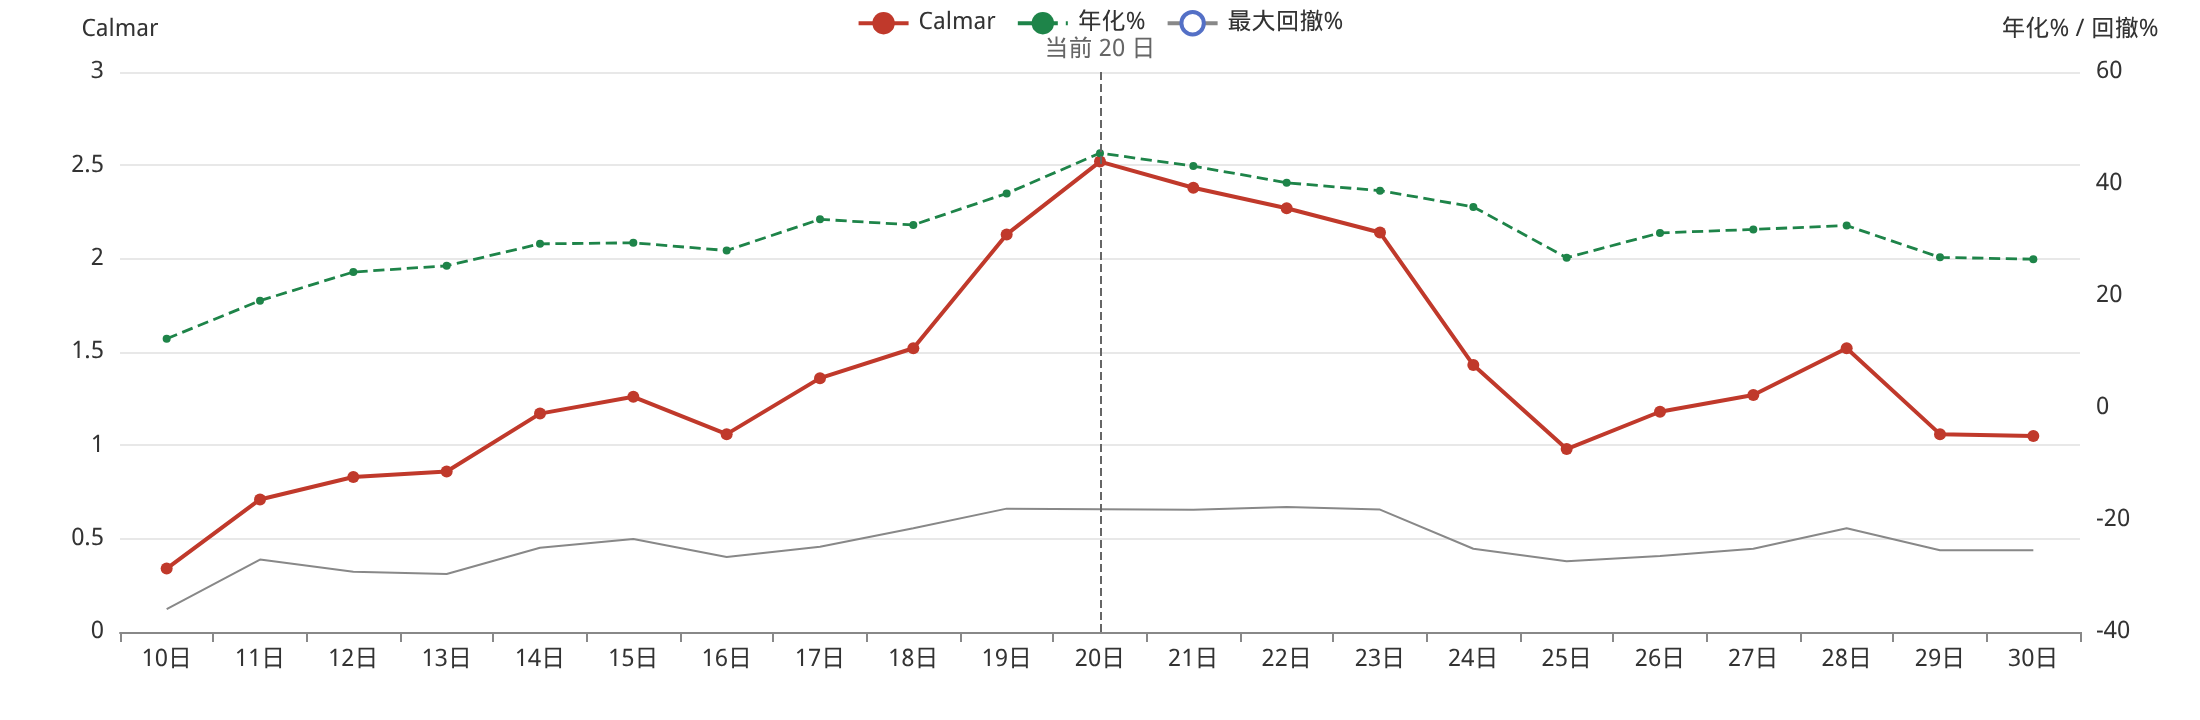
\includegraphics[width=\textwidth]{mom.png}
\caption{动量周期细网格（10$\sim$30 日）：Calmar / 年化 / 最大回撤随周期变化}
\end{figure}

\subsubsection{动量周期细网格（10$\sim$30 日，其余参数固定）}

\begin{table}[htbp]
\centering
\caption{动量周期敏感性（当前 20 日 $\star$）}
\small
\begin{tabular}{rrrrr}
\toprule
动量周期 & 年化 & 最大回撤 & Calmar & 交易 \\
\midrule
10 日 & 12.37\% & $-35.93\%$ & 0.34 & 356 \\
11 日 & 19.17\% & $-27.07\%$ & 0.71 & 333 \\
12 日 & 24.28\% & $-29.25\%$ & 0.83 & 317 \\
13 日 & 25.39\% & $-29.65\%$ & 0.86 & 298 \\
14 日 & 29.31\% & $-24.97\%$ & 1.17 & 304 \\
15 日 & 29.50\% & $-23.41\%$ & 1.26 & 284 \\
16 日 & 28.12\% & $-26.59\%$ & 1.06 & 288 \\
17 日 & 33.69\% & $-24.79\%$ & 1.36 & 262 \\
18 日 & 32.69\% & $-21.47\%$ & 1.52 & 284 \\
19 日 & 38.31\% & $-17.97\%$ & 2.13 & 265 \\
\textbf{20 日（当前）} & \textbf{45.51\%} & \textbf{$-18.08\%$} & \textbf{2.52} & 253 \\
21 日 & 43.20\% & $-18.17\%$ & 2.38 & 245 \\
22 日 & 40.22\% & $-17.69\%$ & 2.27 & 250 \\
23 日 & 38.81\% & $-18.14\%$ & 2.14 & 249 \\
24 日 & 35.91\% & $-25.14\%$ & 1.43 & 262 \\
25 日 & 26.84\% & $-27.37\%$ & 0.98 & 248 \\
26 日 & 31.27\% & $-26.43\%$ & 1.18 & 245 \\
27 日 & 31.89\% & $-25.14\%$ & 1.27 & 251 \\
28 日 & 32.58\% & $-21.47\%$ & 1.52 & 240 \\
29 日 & 26.90\% & $-25.41\%$ & 1.06 & 244 \\
30 日 & 26.57\% & $-25.41\%$ & 1.05 & 233 \\
\bottomrule
\end{tabular}
\end{table}

全样本 Calmar 最优为 \textbf{20 日}（2.52），20 日（当前）排第 1/21 名，10 日档最差。
注意与旧版结论的差异：旧引擎口径下该曲线呈「孤峰」（21 日 2.38，邻档 20=1.98 / 22=1.06）；
当前引擎（QQQ 混合 + 黄金止盈冷却）下已变为 \textbf{18$\sim$22 日的缓坡}——曲线形态本身对引擎口径敏感，
这正是样本特异性的证据，而非参数可靠性的证据。

\subsubsection{其余参数单变量验证（每档格式：年化 / 最大回撤 / Calmar）}

\setlength{\tabcolsep}{4.5pt}
\begin{longtable}{p{2.4cm}p{6.5cm}p{5.9cm}}
\caption{其余参数的单变量扫描}\\
\toprule
参数(当前档) & 档位扫描 & 解读 \\
\midrule
\endfirsthead
\multicolumn{3}{l}{\footnotesize 续表：其余参数的单变量扫描}\\
\toprule
参数(当前档) & 档位扫描 & 解读 \\
\midrule
\endhead
\bottomrule
\endfoot
\footnotesize
止损线 stop\_loss ($-5$ 当前) &
$-3$: 41.77 / $-26.05$ / 1.60；$-5$: 45.51 / $-18.08$ / 2.52；$-8$: 44.52 / $-22.11$ / 2.01 &
$-5\%$ 为峰：$-3\%$ 过紧（回撤 $-23.1\%$），$-8\%$ 过松（$-22.1\%$） \\
\midrule
确认天数 confirm\_days (2 当前) &
1: 45.54 / $-17.11$ / 2.66；2: 45.51 / $-18.08$ / 2.52；3: 43.19 / $-20.39$ / 2.12 &
当前口径下 1$>$2$>$3（1 天档 Cal 2.78）；2 天维持（保守），列入观察 \\
\midrule
快速通道 exception\_gap (3.0 当前) &
2.0: 47.00 / $-18.07$ / 2.60；3.0: 45.51 / $-18.08$ / 2.52；5.0: 44.24 / $-17.69$ / 2.50 &
2.0/5.0 档均略高于 3.0 档；关闭(999)年化 $-4.3$pp \\
\midrule
抄底锁仓 crash\_lock (7 当前) &
5: 45.93 / $-18.08$ / 2.54；7: 45.51 / $-18.08$ / 2.52；14: 46.54 / $-18.08$ / 2.57；21: 45.46 / 2.51；25: 44.41 / 2.46；30: 42.16 / 2.33 &
5$\sim$21 天为平缓高原（14 天微峰），30 天明显变差 \\
\midrule
加速止盈 $\sigma$ accel\_sigma (3.0 当前) &
2.5: 47.08 / $-18.08$ / 2.60；3.0: 45.51 / $-18.08$ / 2.52；3.5: 42.66 / $-24.19$ / 1.76 &
3.0 为峰，两侧下降 \\
\midrule
最短持有 min\_hold (10 当前) &
5: 44.81 / $-18.08$ / 2.48；10: 45.51 / $-18.08$ / 2.52；15: 45.36 / $-17.69$ / 2.56 &
15 天档略优（2.58），稳健 \\
\midrule
最小动量差 min\_gap (1.0 当前) &
0.5: 43.45 / $-18.08$ / 2.40；1.0: 45.51 / $-18.08$ / 2.52；2.0: 45.81 / $-17.69$ / 2.59 &
2.0 档略优（2.56），稳健 \\
\midrule
空仓冷却 sh\_cash\_\allowbreak cooldown (3 当前) &
0: 45.52 / 2.50；1: 45.52 / 2.50；2: 46.25 / 2.61；3: 45.51 / 2.52；4: 43.94 / 2.48；5: 43.07 / 2.43；10: 40.50 / 2.29 &
梯度非单调：2 天档 2.60 最高，3 天档 2.44 为局部低点 \\
\midrule
抄底仓位 crash\_alloc (100 当前) &
50: 43.79 / $-18.08$ / 2.42；100: 45.51 / $-18.08$ / 2.52 &
50\% 档 2.35 vs 全仓 2.44，差异小 \\
\bottomrule
\end{longtable}

\subsection{样本外验证：长样本与两半窗口}\label{sec:oos}

\subsubsection{长样本（2015-01-05 起，含 2015 股灾与 2016 熔断）}

\begin{table}[htbp]
\centering
\caption{长样本稳健性检验（11.6 年）}
\begin{tabular}{lrrrrr}
\toprule
配置 & 累计 & 年化 & 最大回撤 & Calmar & 交易 \\
\midrule
\textbf{当前默认参数} & \pos{6742\%} & 45.74\% & $-21.09\%$ & 2.17 & 284 \\
空仓冷却 0 天 & 5893\% & 44.03\% & $-24.70\%$ & 1.78 & 336 \\
空仓冷却 5 天 & 5441\% & 43.03\% & $-18.07\%$ & 2.38 & 262 \\
$\sigma$ 止损 floor $k=3.0$ & 6606\% & 45.48\% & $-23.73\%$ & 1.92 & 279 \\
\bottomrule
\end{tabular}
\end{table}

把 2015 年股灾与 2016 年初熔断纳入样本后（11.6 年，共 11 次 $>10\%$ 回撤），策略结构与主样本一致。
空仓冷却在该样本上贡献显著（0 天档 Calmar 1.78 vs 3 天档 2.17），5 天档 2.38 略优于 3 天档；
$\sigma$ 止损 floor 在长样本上为 1.92，未复现其旧口径验证期的优势。

\subsubsection{两半窗口 walk-forward（2016--2021 定参 $\rightarrow$ 2021--2026 验证 $\rightarrow$ 2023--2026 压力）}

\begin{center}
\begin{tabular}{p{5.2cm}p{9.6cm}}
\toprule
\textbf{样本内（定参窗）} & \textbf{样本外（验证窗）} \\
\midrule
\small 2016-07-07 $\sim$ 2021-08-20 &
\small 2021-08-23 $\sim$ 2026-08-20 \\
基线：年化 46.31\% / 回撤 $-17.69\%$ / Calmar 2.62 &
基线：年化 43.94\% / 回撤 $-18.34\%$ / Calmar 2.40 \\
最优动量周期(Calmar 前二)：19 日(2.63)、20 日(2.62) &
最优动量周期(Calmar 前二)：22 日(3.54)、23 日(3.20) \\
20 日档：46.31\% / $-17.69\%$ / 2.62 &
20 日档：43.94\% / $-18.34\%$ / 2.40 \\
\midrule
\multicolumn{2}{l}{\textbf{近三年压力窗}（2023-08-21 $\sim$ 2026-08-20）：基线 年化 56.11\% / 回撤 $-17.67\%$ / Calmar 3.18；}\\
\multicolumn{2}{l}{最优动量周期(Calmar 前二)：23 日(6.30)、22 日(6.29)；20 日档：56.11\% / $-17.67\%$ / 3.18} \\
\bottomrule
\end{tabular}
\end{center}

样本外验证窗（2021-08 起）年化 43.94\% 与全样本 45.51\% 基本持平，近三年压力窗年化 56.11\%（含 2025 黄金大牛）。
但最优动量周期从样本内的 19 日漂移至样本外的 22 日——市场节奏在向更长形成期偏移，20 日当前仍稳健，但已不是唯一最优。

\subsection{交易行为解剖：出场通道与恐慌抄底}

\subsubsection{出场通道的成绩单（按平仓原因分组）}

\begin{table}[htbp]
\centering
\caption{各出场通道的收益分布}
\begin{tabularx}{\textwidth}{Xrrrrr}
\toprule
通道 & 笔数 & 胜率 & 平均盈亏 & 中位盈亏 & 合计 \\
\midrule
正常切换 & 25 & 88.0\% & 3.60\% & 2.08\% & 90.00\% \\
$>3\%$切换(快速通道) & 72 & 55.6\% & 2.42\% & 0.64\% & 174.60\% \\
上证空仓(regime 离场) & 41 & 43.9\% & 0.75\% & $-0.20\%$ & 30.80\% \\
加速止盈 & 26 & 69.2\% & 5.72\% & 3.37\% & 148.60\% \\
止损(相对止损) & 3 & 0.0\% & $-6.50\%$ & $-5.85\%$ & $-19.50\%$ \\
绝对止损 & 6 & 0.0\% & $-6.55\%$ & $-6.17\%$ & $-39.30\%$ \\
期末(仍持有) & 1 & 100.0\% & 9.93\% & 9.93\% & 9.90\% \\
\bottomrule
\end{tabularx}
\end{table}

止损/绝对止损通道全亏是\textbf{设计内的保险费}：以确定性小亏交换尾部截断。
正常切换（胜率 88.0\%）与加速止盈是主要利润来源；上证空仓通道合计为正——regime filter 是净增值而非净成本。

\textbf{口径说明（上证空仓胜率 43.9\%）：}该胜率是「离场那一刻这条腿赚没赚钱」的平仓胜率，不是「空仓判断对不对」的准确率。
Regime filter 的本职是「我持有的标的已不再是领导者」时离场，通常贴近盈亏平衡退出（中位 $-0.20\%$），平仓胜率天然偏低。
用最新数据按「离场后 20 个交易日」口径复核：被卖资产平均 $-0.97\%$（中位 $-0.13\%$）——它卖对了资产；
空仓期间净值平均仅变动 $-0.01\%$（几乎零成本）；代价是池内最强资产随后 20 日平均 +6.16\%、63\% 概率涨超 3\%（误伤保费）。
其价值是不对称的：错一次损失几个点的机会成本，对一次（2018-02 volmageddon / 2021-09 / 2026-07 等）躲掉两位数回撤；
消融佐证：关掉该 filter 后 Calmar 2.52$\rightarrow$2.05。

\subsubsection{上证空仓躲过的关键暴跌（逐笔前向审计 · 41 次离场）}

「空仓期收益」= 离场后若继续持有被卖资产、直到下次入场的收益（负值即躲掉的下跌）；
「空仓期最深」= 该期间被卖资产的最大跌幅；「20 日前向」= 离场后 20 个交易日的资产涨跌（验证信号是否命中顶部）。

\begin{table}[htbp]
\centering
\caption{上证空仓逐笔前向审计（代表性事件）}
\small
\begin{tabular}{lllrrr}
\toprule
离场日 & 资产 & 事件背景 & 空仓期收益 & 空仓期最深 & 20 日前向 \\
\midrule
2015-06-08 & 创业 & 2015 股灾顶部(长窗口样本) & \pos{+4.8\%} & $-0.2\%$ & \red{$-40.6\%$} \\
2015-06-15 & 创业 & 2015 股灾第一周(长窗口样本) & \red{$-8.9\%$} & \red{$-11.1\%$} & \red{$-24.3\%$} \\
2017-06-09 & 纳指 & FAANG 科技股回调 & \red{$-4.2\%$} & $-4.2\%$ & \red{$-5.9\%$} \\
2017-07-05 & 创业 & 创业板阴跌(空仓 17 天) & \red{$-6.5\%$} & \red{$-10.8\%$} & \red{$-7.0\%$} \\
2018-02-02 & 纳指 & volmageddon(02-05 VIX 单日飙升) & \red{$-5.4\%$} & \red{$-8.7\%$} & +1.1\% \\
2018-09-21 & 纳指 & Q4 大跌前 7 天离场 & \red{$-1.3\%$} & $-2.9\%$ & \red{$-8.7\%$} \\
2021-02-26 & 纳指 & 成长股杀估值 & \red{$-2.2\%$} & \red{$-5.5\%$} & +1.8\% \\
2021-09-02 & 纳指 & 9 月科技股回调(空仓 20 天) & \red{$-6.0\%$} & \red{$-6.1\%$} & \red{$-6.0\%$} \\
2021-12-06 & 创业 & 年末 A 股调整(空仓 19 天) & \red{$-2.3\%$} & \red{$-6.1\%$} & $-4.3\%$ \\
2023-04-20 & 创业 & 4 月 A 股调整 & \red{$-5.2\%$} & \red{$-5.2\%$} & \red{$-5.5\%$} \\
2023-08-07 & 创业 & 8 月 A 股下跌 & \red{$-4.1\%$} & $-4.1\%$ & \red{$-5.4\%$} \\
2025-03-07 & 创业 & 顶部命中(离场后 20 日 $-17.8\%$) & \red{$-2.2\%$} & $-3.4\%$ & \red{$-17.8\%$} \\
2026-03-05 & 黄金 & 黄金回调 & \red{$-3.0\%$} & $-3.1\%$ & \red{$-11.2\%$} \\
2026-07-02 & 创业 & 2026-07 A 股暴跌 & \red{$-7.1\%$} & \red{$-7.2\%$} & \red{$-19.0\%$} \\
\bottomrule
\end{tabular}
\end{table}

合计口径：主窗口 41 次离场中，「20 日前向 $\le-5\%$（躲对）」\textbf{10 次}、「$\ge+5\%$（卖飞）」\textbf{4 次}、其余 27 次中性（多在 $\pm2\%$ 内）；
若每次离场后都傻等被卖资产到下次入场，十年累计多亏 $-23.9\%$。
典型的躲过包括 2018-02 波动率崩溃、2021-09 科技股回调、2023-04/08、2026-03 黄金与 2026-07 A 股两连击——且 2025-03 与 2015-06 两次都精确踩在顶部。

\textbf{能力边界}：它躲的是「领导力背离型」顶部，不是全部系统性危机——2020-03 疫情崩盘期间该 filter 零触发（靠止损 + 恐慌抄底兜底）；
2016-01 熔断也是先误报（2015-12-25 离场黄金）后于熔断首日再入场，未躲成。
它也时常「躲了开头就回来」（2025-03 再入场过早，只吃到 $-2.2\%$）——冷却 3 天挡不住规则化的再入场，这是它与「全程躲熊市」择时器的本质区别。
最大卖飞：2022-05-27 离场创业后 20 日 +21.8\%。

\subsubsection{恐慌抄底逐笔记录（8 笔已平仓）}

\begin{table}[htbp]
\centering
\caption{恐慌抄底逐笔明细}
\begin{tabular}{llrrl}
\toprule
入场日 & 出场日 & 盈亏 & 持有天数 & 出场方式 \\
\midrule
2018-02-09 & 2018-04-11 & \pos{15.09\%} & 36 天 & $>3\%$切换 \\
2018-10-18 & 2018-10-29 & \pos{3.36\%} & 7 天 & $>3\%$切换 \\
2020-03-18 & 2020-03-27 & \pos{0.64\%} & 7 天 & $>3\%$切换 \\
2021-03-09 & 2021-03-18 & \pos{4.02\%} & 7 天 & $>3\%$切换 \\
2022-03-15 & 2022-03-24 & \pos{8.20\%} & 7 天 & $>3\%$切换 \\
2022-04-26 & 2022-05-10 & \pos{5.64\%} & 7 天 & $>3\%$切换 \\
2025-04-07 & 2025-04-16 & \pos{5.33\%} & 7 天 & $>3\%$切换 \\
2026-07-17 & 2026-07-28 & \red{$-3.14\%$} & 7 天 & $>3\%$切换 \\
\bottomrule
\end{tabular}
\end{table}

\subsection{持仓结构：分标的持有时间 / 收益分布 / 持仓占比}

全样本 2459 个交易日中，持仓 2067 天（84.1\%）、空仓 73 段共 392 天（15.9\%，空仓段中位 3 天、最长 35 天）；
共 179 段持仓，平均每段持有 11.5 个交易日。

\begin{table}[htbp]
\centering
\caption{分标的持仓结构与收益贡献}
\footnotesize
\resizebox{\textwidth}{!}{%
\begin{tabular}{lrrrrrrrrrrrrr}
\toprule
标的 & 持仓段数 & 时间占比 & 均持有 & 中位持有 & 最长持有 & 平均收益 & 中位收益 & 收益贡献 & 贡献占比 & 胜率 & 收益分布 & 持有天数分布 \\
\midrule
创业 & 63 & 28.0\% & 10.9 & 7 & 72 & 3.60\% & 1.15\% & \pos{+226.6pp} & \pos{+56.0\%} & 57.1\% & 4/23/17/9/10 & 24/19/11/8/1 \\
纳指 & 62 & 36.2\% & 14.4 & 6 & 85 & 2.47\% & 1.88\% & \pos{+152.8pp} & \pos{+37.8\%} & 64.5\% & 4/18/24/11/5 & 28/6/15/8/5 \\
黄金 & 54 & 19.8\% & 9.0 & 6 & 42 & 0.46\% & 0.43\% & \pos{+24.9pp} & \pos{+6.2\%} & 50.0\% & 2/25/21/5/1 & 26/14/8/5/1 \\
\bottomrule
\end{tabular}}
\end{table}

\begin{quote}\footnotesize
\textbf{口径}：每段持仓 = 买入/切换入 $\rightarrow$ 卖出/切换出/期末持有的完整腿；收益为段内净值盈亏（含手续费），期末持仓段计入；
收益贡献 = 各段盈亏(pp)之和，贡献占比 = 该标的总盈亏 / 全池总盈亏；时间占比 = 该标的持有交易日 / 全样本交易日。
收益分布与持有天数分布列的分桶分别为（$\le-5$ / $-5\sim0$ / $0\sim5$ / $5\sim10$ / $>10$）与（1-5 / 6-10 / 11-20 / 21-40 / 40+）。
\end{quote}

\begin{figure}[htbp]
\centering
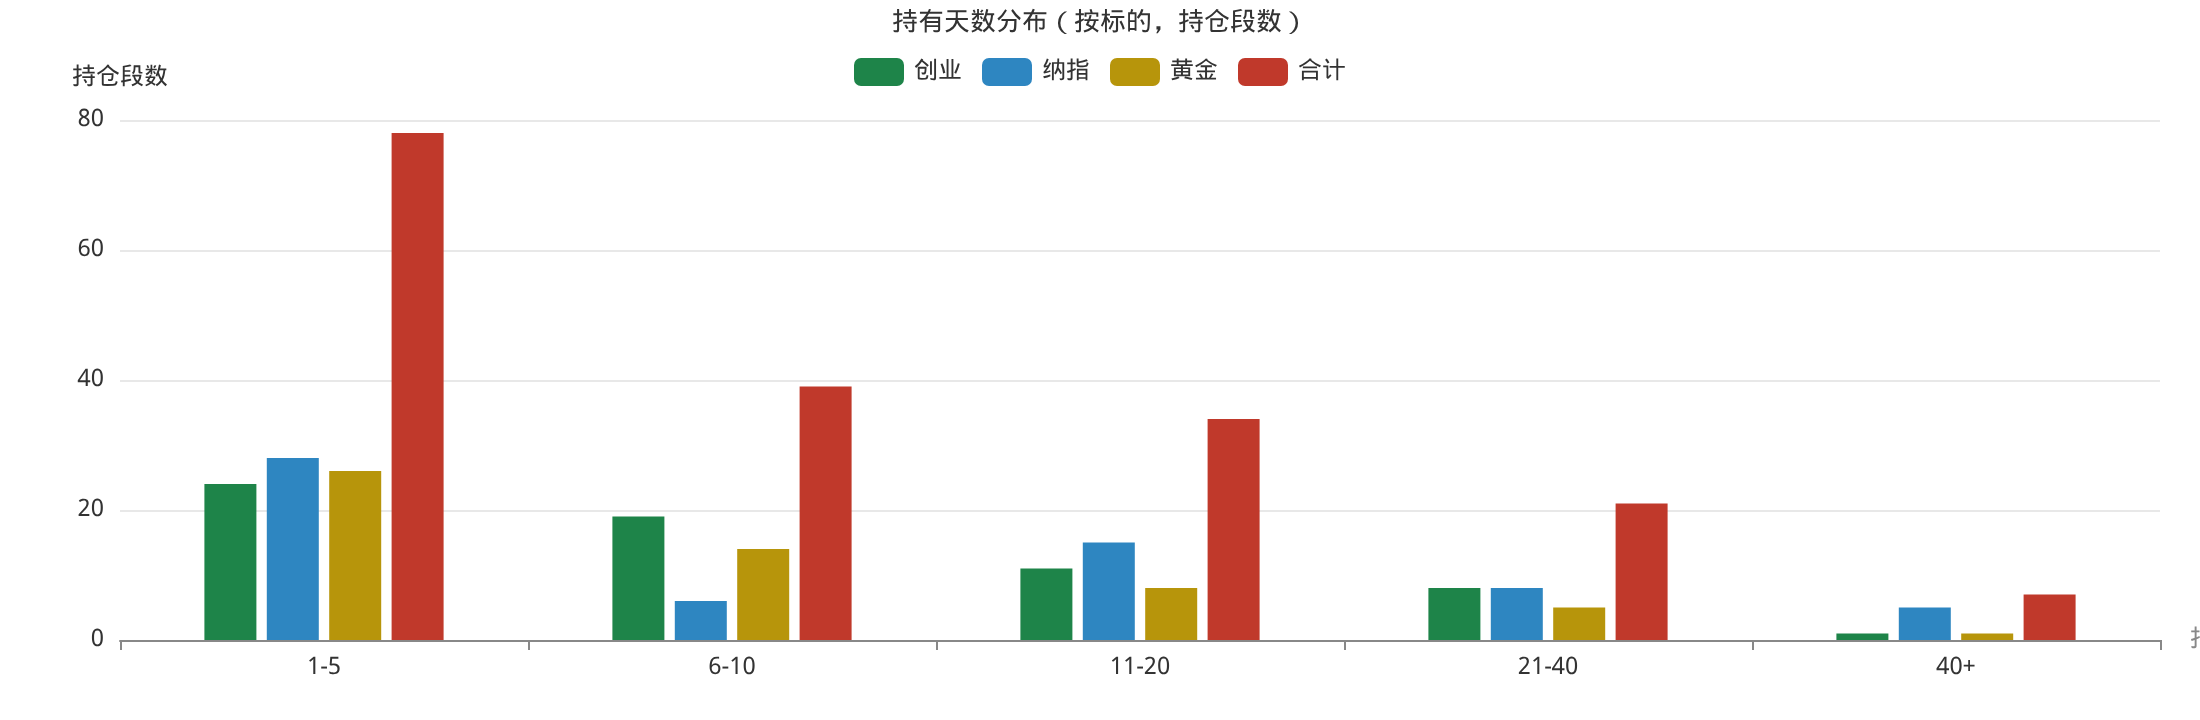
\includegraphics[width=0.86\textwidth]{hold_days.png}
\caption{持有天数分布（按标的，持仓段数）}
\end{figure}

\begin{figure}[htbp]
\centering
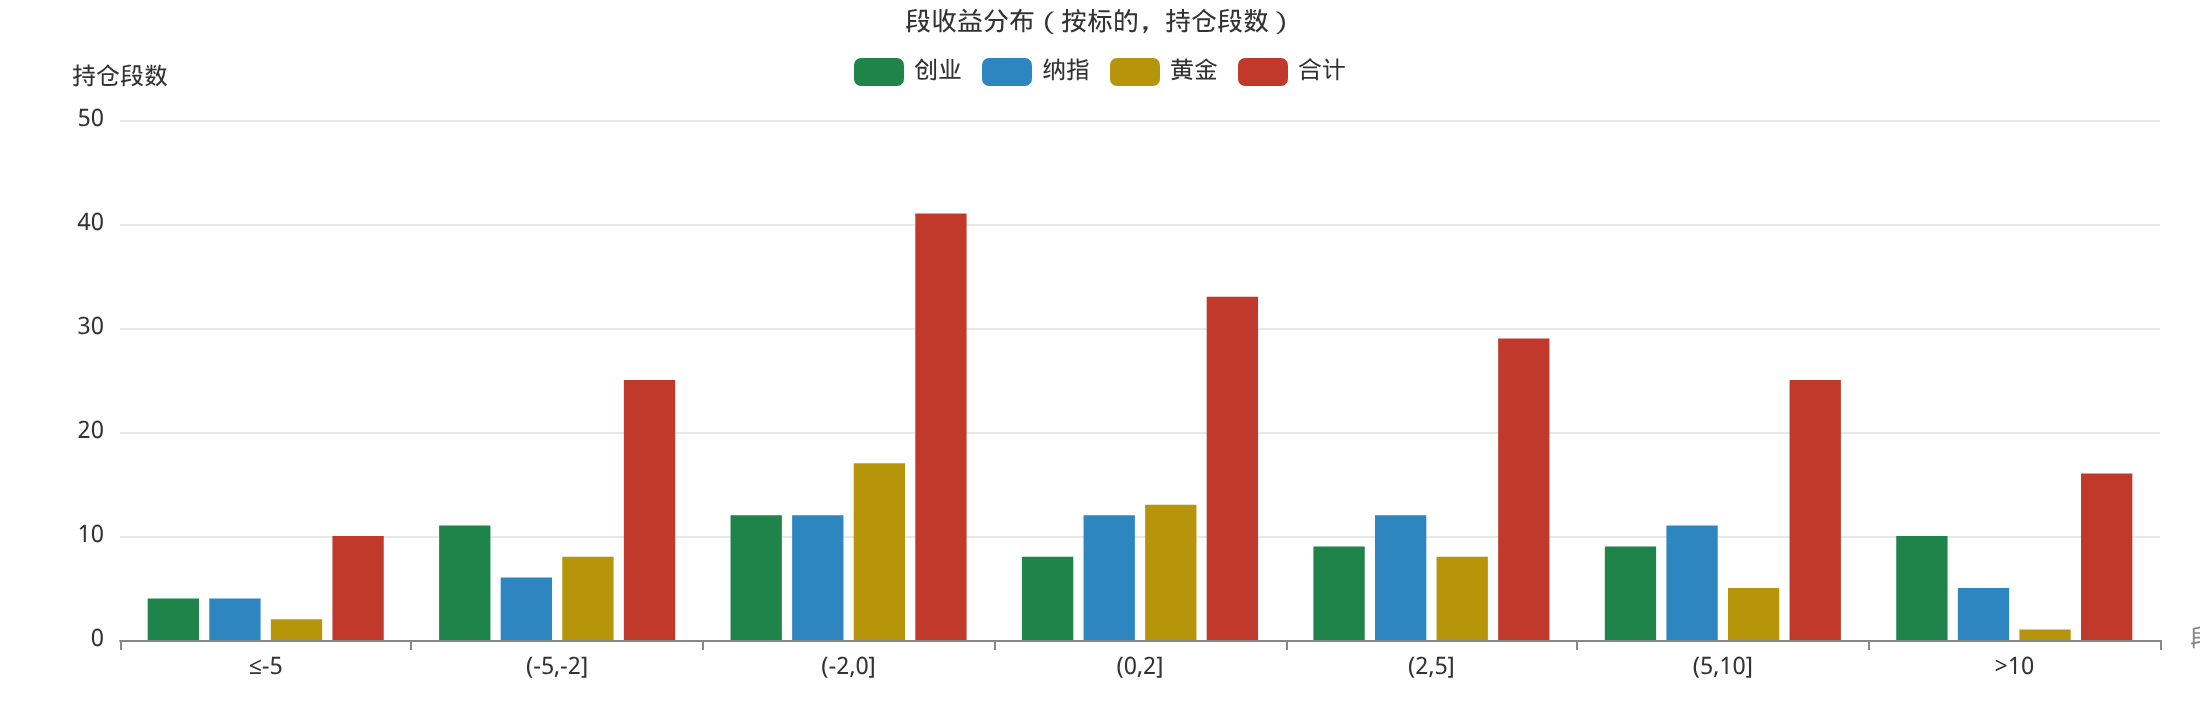
\includegraphics[width=0.86\textwidth]{hold_pnl.png}
\caption{段收益分布（按标的，持仓段数）}
\end{figure}

\subsection{成本敏感性}

\begin{table}[htbp]
\centering
\caption{单边交易成本（佣金+滑点）的敏感性}
\begin{tabular}{lrrrrr}
\toprule
单边成本 & 累计 & 年化 & 最大回撤 & Calmar & 交易 \\
\midrule
基线(仅手续费 0.01\%) & 3785\% & 45.51\% & $-18.08\%$ & 2.52 & 253 \\
0.05\% & 3150\% & 42.87\% & $-19.54\%$ & 2.19 & 253 \\
0.1\% & 2618\% & 40.28\% & $-20.98\%$ & 1.92 & 253 \\
0.2\% & 1801\% & 35.23\% & $-23.77\%$ & 1.48 & 253 \\
\bottomrule
\end{tabular}
\end{table}

十年约 253 次交易（买+卖），滑点对复利影响显著：每 0.1\% 单边滑点约削去 5.2pp 年化。
ETF 实际冲击成本接近零，实盘评估建议按 0.05\% 滑点口径。

\subsection{加仓时机研究：立即追 vs 等下一次调仓（2026-08-21/23）}

\textbf{方法}：复用生产回测引擎，在全历史每个交易日模拟一笔加仓，比较 A「立即按当前持仓买入」、
B「等策略第一次调仓再进」、D「10 日均分」三种方式在同一持有窗口 [注入日, 注入日+H] 的收益（A$-$B 为两者收益差，pp）。

\subsubsection{总体（各持有期口径）}

\begin{table}[htbp]
\centering
\caption{三种加仓方式的持有期收益对比}
\footnotesize
\setlength{\tabcolsep}{3.8pt}
\begin{tabular}{lrrrrrrr}
\toprule
持有期 & 样本 & A 胜率 & A$-$B 平均 & A$-$B 中位 & A 均收益 & B 均收益 & D 均收益 \\
\midrule
1 个月 & 2048 & 61.9\% & \pos{1.92pp} & 0.88pp & 3.36\% & 1.44\% & 2.38\% \\
3 个月 & 2017 & 62.0\% & \pos{2.63pp} & 0.94pp & 10.23\% & 7.60\% & 9.18\% \\
6 个月 & 1965 & 61.8\% & \pos{2.72pp} & 1.01pp & 21.17\% & 18.44\% & 20.05\% \\
12 个月 & 1854 & 62.7\% & \pos{3.60pp} & 1.37pp & 51.82\% & 48.22\% & 50.39\% \\
\bottomrule
\end{tabular}
\end{table}

\subsubsection{按「注入时当前持仓收益率」分档（12 个月口径）}

\begin{table}[htbp]
\centering
\caption{加仓时点分档：立即追(A) vs 等调仓(B) vs 均分(D)}
\small
\begin{tabular}{lrrrrrrl}
\toprule
当前持仓浮盈亏 & 样本 & A 胜率 & A$-$B 平均 & A 均收益 & B 均收益 & D 均收益 & 推荐 \\
\midrule
($-5$,$-2$]\% & 78 & 65.4\% & \pos{1.43pp} & 63.34\% & 61.90\% & 62.51\% & 立即追 \\
($-2$,0]\% & 430 & 56.3\% & \pos{3.16pp} & 54.47\% & 51.31\% & 52.99\% & 立即追 \\
(0,2]\% & 382 & 69.1\% & \pos{4.27pp} & 50.54\% & 46.27\% & 49.22\% & 立即追 \\
(2,5]\% & 406 & 68.2\% & \pos{4.28pp} & 51.40\% & 47.13\% & 49.53\% & 立即追 \\
(5,10]\% & 309 & 59.5\% & \pos{3.87pp} & 50.06\% & 46.19\% & 48.49\% & 立即追 \\
$>10\%$ & 249 & 57.8\% & \pos{2.59pp} & 48.48\% & 45.89\% & 47.67\% & 立即追 \\
\bottomrule
\end{tabular}

\small 注：$\le-5\%$ 档样本为 0——策略绝对止损在 $-5\%$ 清仓，收盘口径下不存在「深亏超 5\% 仍持仓」的加仓时点。
\end{table}

\begin{itemize}
  \item \textbf{每一档都是「立即追」赢}——「无脑追」的结论经得起收益率分档检验，四个月口径方向一致，无任何档位反转。
  \item 优势呈\textbf{倒 U 型}：刚转正(0$\sim$5\%)档最优(+4.3pp、胜率 68$\sim$69\%)——策略刚确认趋势时追仓最划算；浮亏档次之；大涨后($>10\%$)减弱到 +2.6pp（离加速止盈更近，等待代价变小）。
  \item 不利尾部几乎全压在「等调仓」一侧：等调仓吃大亏($\ge5$pp)概率 28.5\% 是占大便宜(6.8\%)的 4.2 倍，且有 24.9\% 概率一个月等不到调仓。
  \item 大额资金心理压力大时，D（10 日均分）期望接近 A，是低后悔的折中。
\end{itemize}

\begin{quote}\footnotesize
\textbf{口径}：空仓注入日 A$\equiv$B 已剔除；收益为净值口径含手续费；\\
完整明细与脚本见 backtest/add\_capital\_entry.py、add\_capital\_entry\_result.json、加仓时机分析.md。
\end{quote}

% ═══════════════ 5 讨论 ═══════════════
\section{讨论}

\subsection{结构上的优势}

\begin{itemize}
  \item \textbf{Regime filter 是灵魂。}「上证动量强于池内最强即离场」检测的是领导力背离——宽基走强而策略池不参与，历史上多次关键顶部均有触发（2015-06/12 股灾顶部、2018-02 volmageddon、2021-09、2026-07 等，见 4.5 节）。它用择时代替分散做风控：这也是 Top-2 分散实验为大幅负优化的原因——风控已被 filter 承担，分散只稀释 alpha。
  \item \textbf{两端均值回归叠加补齐动量短板。}动量策略在顶部追高、底部割肉；加速止盈卖在高潮、恐慌抄底买在恐慌，精确对冲这两个固有缺陷。
  \item \textbf{成本纪律到位。}确认天数/最短持有/最小动量差抑制换手，手续费独立建模并做压力测试。
\end{itemize}

\subsection{脆弱点与红旗}\label{sec:fragile}

\begin{itemize}
  \item \textbf{动量周期的跨期漂移。}全样本最优 19 日、当前用 20 日；样本内窗最优 19 日、样本外窗漂移到 22 日（4.4 节）。当前引擎下曲线虽已从「孤峰」变为缓坡，但最优值随样本移动——这是\textbf{样本特异性共振}的痕迹，不是结构性 alpha。
  \item \textbf{选池偏差未被完全分解。}纳指与黄金恰是这十年全球最强的两类资产，年化收益中相当部分是「选对池」而非轮动 alpha。等权买入持有对照（4.1 节）已控制掉一部分，但池内替代性（如创业板$\rightarrow$沪深300）的对照仍是遗留空白。
  \item \textbf{全参数样本内选择。}20 日、$3\sigma$、$-2.5\sigma$、3 天冷却……全部选自主样本。两半窗口验证（4.4 节）是部分解药，且确实显示最优参数随窗口漂移。
  \item \textbf{用上证当全球 regime 锚是集中押注。}池中 3 个资产有 2 个（纳指/黄金）与 A 股相关性有限，但总风控开关绑在上证动量上。若下一次危机是美国特有而 A 股无恙，filter 可能不触发。
  \item \textbf{二元全仓、无仓位管理。}每次回撤都足额承受；波动率目标化（TSMOM 式缩放）是未实现的理论改进方向。
\end{itemize}

\subsection{与上一版分析的差异（结论变更记录）}

\begin{table}[htbp]
\centering
\caption{结论变更记录}
\small
\begin{tabular}{p{2.8cm}p{4.6cm}p{7.6cm}}
\toprule
议题 & 旧结论(2026-08 早期) & 当前状态 \\
\midrule
纳指动量信号源 & 纯 513100 ETF 价格动量 & \textbf{已改为 $0.7\times$QQQ-CNY + $0.3\times$ETF 混合}(I-11 决议)：回退纯 ETF 口径 Calmar 从 2.52 降至 1.99。 \\
止盈后冷却 & 默认关闭(历史判定负优化) & \textbf{已改为黄金止盈后冷却 3 天}(I-15/16/17 决议)：回退后全样本 Calmar 升至 2.67 但 2025 年 $-16.2$pp，决议基于近期证据维持；扩至全部标的为负优化(1.85)。 \\
2026-06$\sim$07 连环止损段 & 十年最深回撤 $-25.7\%$ & 当前口径下该段回撤 $-11.92\%$（谷底 2026-07-30），最深度让位于 2025-09$\sim$2026-04 段。 \\
动量周期曲线 & 20/21 日孤峰(邻档断崖) & 当前口径下为 18$\sim$22 日缓坡，全样本最优 19 日；样本外最优漂移至 22 日。 \\
$\sigma$ 自适应止损 floor $k=3.0$ & 2026-08-14 三窗口验证通过后落地实盘 & 实盘已部署(stock-bot cron)；当前默认口径 + 最新数据下为负优化(主样本 1.81 vs 基线 2.52)，列观察项。 \\
扩池 & 3$\rightarrow$4$\rightarrow$8$\rightarrow$14 池单调恶化，写入纪律 & 维持窄池 3，未重验。 \\
\bottomrule
\end{tabular}
\end{table}

% ═══════════════ 6 结论 ═══════════════
\section{结论与实盘含义}

\begin{enumerate}
  \item 策略在十年主样本上取得年化 \textbf{45.51\%}、最大回撤 \red{$-18.08\%$}、Calmar \textbf{2.52}，11 个年份中仅 2016 年为负；该结果在长样本（2015 起）与样本外窗口（2021 起）中方向一致、幅度相当。
  \item 收益结构可分解：窄池相对动量（引擎）+ regime filter（锚）+ 两端风控（保险与增强）。消融证实各模块不可删除；教科书式「改进」（分散持仓、多周期动量、动量跳过）为大幅负优化，波动率归一/防御切换/FIP 为中性偏负——\textbf{集中持仓与窄池是设计而非缺陷}。
  \item 参数体系整体稳健，主要红旗是动量周期的跨期漂移（样本内 19 日 $\rightarrow$ 样本外 22 日）。合理的长期预期不是点估计 45.51\%，而是 \textbf{30\%$\sim$45\% 年化、$-18\%\sim-25\%$ 回撤}的区间。
  \item 实盘含义：维持当前默认参数；换参的触发条件应是 21/22 日档在实盘持续反超 20 日档（而非回测网格）；已部署的 $\sigma$ 止损 floor 变体在当前口径下未复现其验证期优势，列为观察项。
\end{enumerate}

\begin{quote}\small
本报告所有数字由 web/bt\_runner.run\_backtest 在 2026-08-20 数据上重跑生成（完整结果 audit/out/paper\_2026.json，生成脚本 audit/paper\_experiments.py）；
历史研究结论存档 audit/审计结果清单.md。本报告与线上分析页（web/templates/analysis.html）内容一致，以本 LaTeX 版本为准。
\end{quote}

\end{document}
